\documentclass{article}
\usepackage{graphicx}
\usepackage[utf8]{inputenc}
\renewcommand{\baselinestretch}{1.2} 
\title{\textbf{Artificial Intelligence Methods for Complex Industrial Scheduling Applications} \\}


\author{\\[1in] Student: \\ \textit{\textbf{Mohammed El-Kholany, MSc.}}\\Alpen-Adria-Universität Klagenfurt, Austria \\[1in] \and Supervisor:\\ \textit{\textbf{Prof. Martin Gebser}} \\ \and
Co-supervisor:\\ \textit{\textbf{Assoc. Prof. Konstantin Schekotihin}} \\[1in]}
\date{December 2020}

\begin{document}

\clearpage\maketitle
\thispagestyle{empty}
\clearpage
\setcounter{page}{1}
\newpage
\section{Introduction}
The study of production systems is complex, given a large number of integrated entities and interactions. This complexity is one of the scheduling problem causes, which are generally recognized as difficult to solve\cite{garey1979computers,lenstra1977complexity}. Scheduling of operations involves resource allocation over a period of time to perform a series of tasks. There are several types of scheduling problems, one of the most critical problems is the Job-Shop Scheduling Problem (JSP). The JSP has been known as a notoriously complex and stubborn combinatorial optimization problem since the 1950s, and it has been proven to be NP-hard in \cite{baker1974introduction,lenstra1979computational}. Therefore, it was very difficult to reach the optimal solution, even for small-scale instances.\\

However, in the practical manufacturing environment, the Job-Shop Scheduling Problem scale is much larger, where the number of operations may be up to 10000 in some mechanical workshops \cite{zhang2010hybrid}. The main purpose is to find the most appropriate sequencing of operations on the machines to optimize the performance indicator. A typical performance indicator for JSP is the makespan, which is the time needed to complete all jobs. \\

The real world is subject to many change sources, typically treated as random occurrences such as breakdown machines, new job arrivals, change in due dates, and canceling orders. These random occurrences might cause some disturbances and make the original schedule infeasible in \cite{salido2017rescheduling}. Many researchers focused on Dynamic Job-shop Scheduling Problem (DJSP) to handle unforeseen events \cite{zhang2017flexible,xiong2013robust, salido2017rescheduling}. It is a NP-hard optimization problem and a computationally challenging issue. \\

In DJSP, urgent jobs can arrive at some unknown times. The generated schedules may become outdated when they are inserted to the shop floor. Since it is difficult to take into account these changes while generating a schedule. A rescheduling strategy is necessary to update the production schedule and guarantee feasibility and efficiency. The dynamic scheduling is the process of generating a schedule based on the old one to respond to disturbances \cite{sajadi2019robust}. DJSP applications can be found in different real-world applications such as production planning, machine scheduling, etc. This makes DJSP attracted much attention from a significant number of researchers and many heuristics and meta-heuristics that have been proposed to find a near-optimal solution for DJSP. 

\section{State of the art}
Since the JSP has NP-hard property, the performance of traditional methods will hardly be satisfactory. To overcome these difficulties, several decomposition-based algorithms have been proposed. The main idea of the decomposition approach is to divide the original problem into a series of smaller sub-problems and solve sub-problems respectively to obtain the final solution of the original problem. For instance, a decomposition-based hybrid approach for solving large-scale JSP is proposed in \cite{zhang2010hybrid} while the total weighted tardiness must be minimized. In each iteration, a sub-problem is defined using Simulated Annealing and solved by a Genetic Algorithm. \\

In \cite{zhai2014decomposition}, a new method for detecting multi-bottleneck machines is proposed where the characteristics of bottleneck machines are used to improve the solution efficiency. As mentioned in the previous section, handling unforeseen events like (breakdown machines, the arrival of urgent jobs, and canceling orders) is one of the most critical success keys in the manufacturing systems. \\

For this reason, many researchers have tackled DJSP while minimizing the effect of disruptions that might occur. Most of the schedules consider only shop efficiency. However, when a disruption occurred a new generated schedule might deviate significantly from the original one, and it can seriously affect the floor's performance. The main objective of dynamic scheduling is to generate a new schedule based on the old one considering the shop efficiency (makespan minimization) and stability (minimizing the deviation from the original schedule) \cite{ouelhadj2009survey}. Three different rescheduling strategies: Right-Shift Rescheduling, Fixed-Sequence Rescheduling, and Total Rescheduling have been studied in \cite{mason2004rescheduling}, while investigating each strategy's efficacy to minimize the total weighted tardiness. The experiments showed that breakdown machine time is sensitive to rescheduling performance.\\

A new rescheduling strategy based on the Genetic Algorithm and tabu search is proposed to solve the DJSP where the objective is to minimize the makespan in \cite{ali2019adopted}. This study investigated the arrival of new jobs unconditionally at the system. Another version of the Genetic Algorithm has been developed to solve JSP with machine disruptions in \cite{wang2013novel} while minimizing the makespan. We see that the previous studies aimed to optimize the shop's efficiency and considered only one disruption. Some studies tackled a different kind of disruption in addition to optimizing schedule efficiency and schedule stability simultaneously. For instance, a rescheduling approach based on the Genetic Algorithm and tabu search has been presented to solve the DJSP with machine breakdowns and random job arrivals in \cite{zhang2013hybrid}. The proposed algorithm aimed to generate a robust and stable schedule by minimizing the makespan and the starting time deviations of the operations simultaneously. 

\section{Problem Statement}
In the JSP, the problem consists of $n$ jobs and a set of $m$ machines. Each job has a series of operations. The operations must be executed sequentially and need to be processed on specific machines. Each machine can process only one operation at a time. The Dynamic JSP is an extension of the JSP, and the execution of a schedule is usually confronted with disruptions and unforeseen events. Many real-time events could occur during the scheduling process, such as random job arrivals, machine breakdowns, and cancel orders. When an unforeseen event happens, the system should react and update the schedule very fast to adapt with the new situation.
\subsection{Research Questions}
\begin{enumerate}
    \item What is the most appropriate decomposition method to solve JSP and obtain near optimal solution in a reasonable time?
    \item How to develop an efficient method that generates a robust schedule?
    \item How to build a framework that finds a robust and stable predictive schedule to handle unforeseen events?
\end{enumerate}

\section{Contribution}
In summary, the number of papers on the Dynamic Job-shop scheduling problem has been increasingly growing in recent years. However, most of them were tackling schedule efficiency that implies high machine utilization. It can improve shop efficiency. However, the schedule that only considers the schedule efficiency may deviate from the original schedule. It can have a negative impact on shop performance.
Moreover, most of the work focused on small-scale benchmark instances considering only an unexpected event, which does not fit real applications in the production systems. Therefore, it is essential to study Dynamic JSP by considering the schedule efficiency and schedule stability simultaneously. This thesis aims to develop an enhanced framework that provides a robust and stable schedule to solve large-scale instances and considers different unexpected events (breakdown machines, the arrival of new jobs, and canceling orders). 
More preciously, the research objectives of this Ph.D. are:
\begin{enumerate}
    \item This package aims to develop an efficient approach that decomposes the JSP into a series of sub-problems and obtain near-optimal solutions in a reasonable time. To evaluate our proposed approach, we should perform many experiments on large-scale instances to validate its efficiency.
    \item Secondly, we will consider machine breakdown and develop a technique that minimizes the classical performance measure (makespan). In this phase, we will focus only on minimizing the makespan's deviation.
    \item The third objective is to provide a robust and stable schedule that optimizes the second research objective and minimizes the deviation of the operations' starting time and the sequence of the operations.
    \item The last objective of this Ph.D. project is to consider two other types of disruptions: the arrival of new jobs and canceling orders while optimizing the same objectives.
\end{enumerate}

\section{Methodology}
We plan to build our models using Answer Set Programming (ASP), a programming methodology rooted in artificial intelligence and computational logic research \cite{lifschitz2002answer}. It is considered among the most popular paradigms for knowledge representation and reasoning, especially in combinatorial optimization problems \cite{abseher2016shift}. ASP was successfully used in various application areas, including team building and scheduling \cite{ricca2011team}, bio-informatics \cite{guziolowski2013exhaustively}, and product configuration \cite{soininen1999developing}. An ASP program contains logic rules, including variables and facts, which represent the input. Standard ASP follows a one-shot process in computing answer set(s) of a logic program, and then a new flexible paradigm of grounding and solving is proposed, which is multi-shot ASP solving \cite{gebser2019multi}. The Multi-shot ASP deals with continuously changing logic programs, and it allows for advanced forms of search as in optimization problems.

\section{Progress and Schedule}
In October 2019, we started by doing an extensive review of the JSP papers that have been published recently. After reviewing the articles, we develop a single-shot ASP model to solve the JSP problem in January. Because of the results' limitations, we developed several techniques that decompose the problem into time windows and solve the problem using multi-shot ASP. The preliminary results were accepted as an extended abstract in workshop TAASP 2020. By submitting the extended results as a journal/conference paper, the first objective will be finalized in February 2021. The next step is to start working on the second objective, which is planned to be finished by December 2021. As the last two objectives are correlated, the fourth objective will be overlapped with the third objective, and the thesis will be completed in June 2023. 

\begin{figure}[h!]
  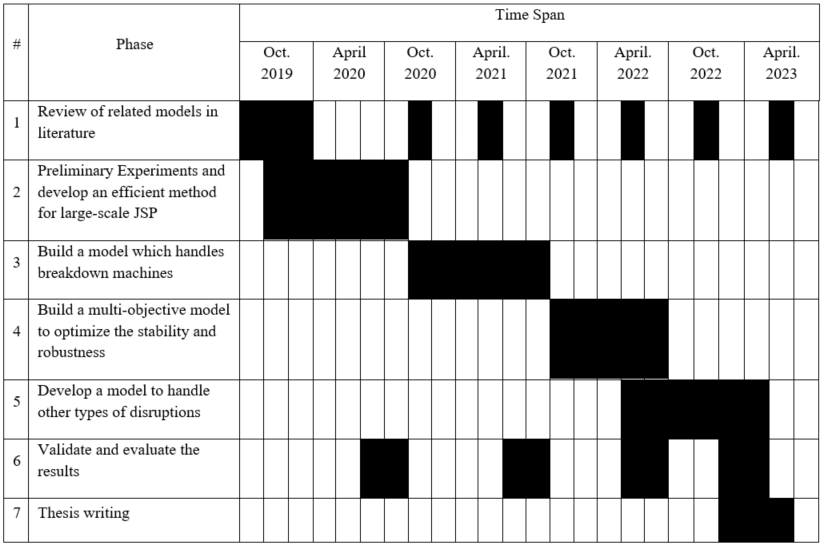
\includegraphics[width=\linewidth]{Plan2.png}
  \caption{Work plan.}
  \label{fig:Work plan}
\end{figure}
\newpage
\bibliographystyle{ieeetr.bst}
\bibliography{references.bib}
\end{document}

